\section{Resultados}

\subsection{Ejercicio 1: Matriz de Leontief Básica}

En este ejercicio se calculó la matriz de coeficientes técnicos, la matriz inversa de Leontief, la producción total requerida y los multiplicadores de producción para los tres sectores de la economía de La Guajira.

\subsubsection{Matriz de Coeficientes Técnicos (A)}

La matriz de coeficientes técnicos muestra los requerimientos de insumos por unidad de producción para cada sector:

\begin{table}[H]
\centering
\caption{Matriz de Coeficientes Técnicos (A)}
\begin{tabular}{lccc}
\toprule
 & Agricultura & Tecnología & Servicios \\
\midrule
Agricultura & 0.100 & 0.133 & 0.023 \\
Tecnología & 0.160 & 0.167 & 0.154 \\
Servicios & 0.120 & 0.111 & 0.192 \\
\bottomrule
\end{tabular}
\end{table}

La interpretación de estos coeficientes indica que, por ejemplo, para producir una unidad de Agricultura se requieren 0.100 unidades de Agricultura, 0.160 unidades de Tecnología y 0.120 unidades de Servicios.

\subsubsection{Matriz Inversa de Leontief $(I - A)^{-1}$}

La matriz inversa de Leontief muestra los efectos directos e indirectos de los cambios en la demanda final:

\begin{table}[H]
\centering
\caption{Matriz Inversa de Leontief $(I - A)^{-1}$}
\begin{tabular}{lccc}
\toprule
 & Agricultura & Tecnología & Servicios \\
\midrule
Agricultura & 1.155 & 0.194 & 0.070 \\
Tecnología & 0.260 & 1.275 & 0.250 \\
Servicios & 0.207 & 0.204 & 1.283 \\
\bottomrule
\end{tabular}
\end{table}

\subsubsection{Producción Total Requerida}

La producción total requerida para satisfacer la demanda final es:

\begin{table}[H]
\centering
\caption{Producción Total Requerida por Sector}
\begin{tabular}{lc}
\toprule
Sector & Producción (miles de millones de pesos) \\
\midrule
Agricultura & 4.80 \\
Tecnología & 7.88 \\
Servicios & 11.70 \\
\bottomrule
\end{tabular}
\end{table}

\subsubsection{Multiplicadores de Producción}

Los multiplicadores de producción indican el impacto total (directo e indirecto) de cada sector:

\begin{table}[H]
\centering
\caption{Multiplicadores de Producción por Sector}
\begin{tabular}{lc}
\toprule
Sector & Multiplicador \\
\midrule
Agricultura & 1.62 \\
Tecnología & 1.67 \\
Servicios & 1.60 \\
\bottomrule
\end{tabular}
\end{table}

El sector Tecnología presenta el mayor multiplicador (1.67), lo que indica que un aumento en su demanda final genera el mayor impacto sobre el conjunto de la economía.

\begin{figure}[H]
\centering
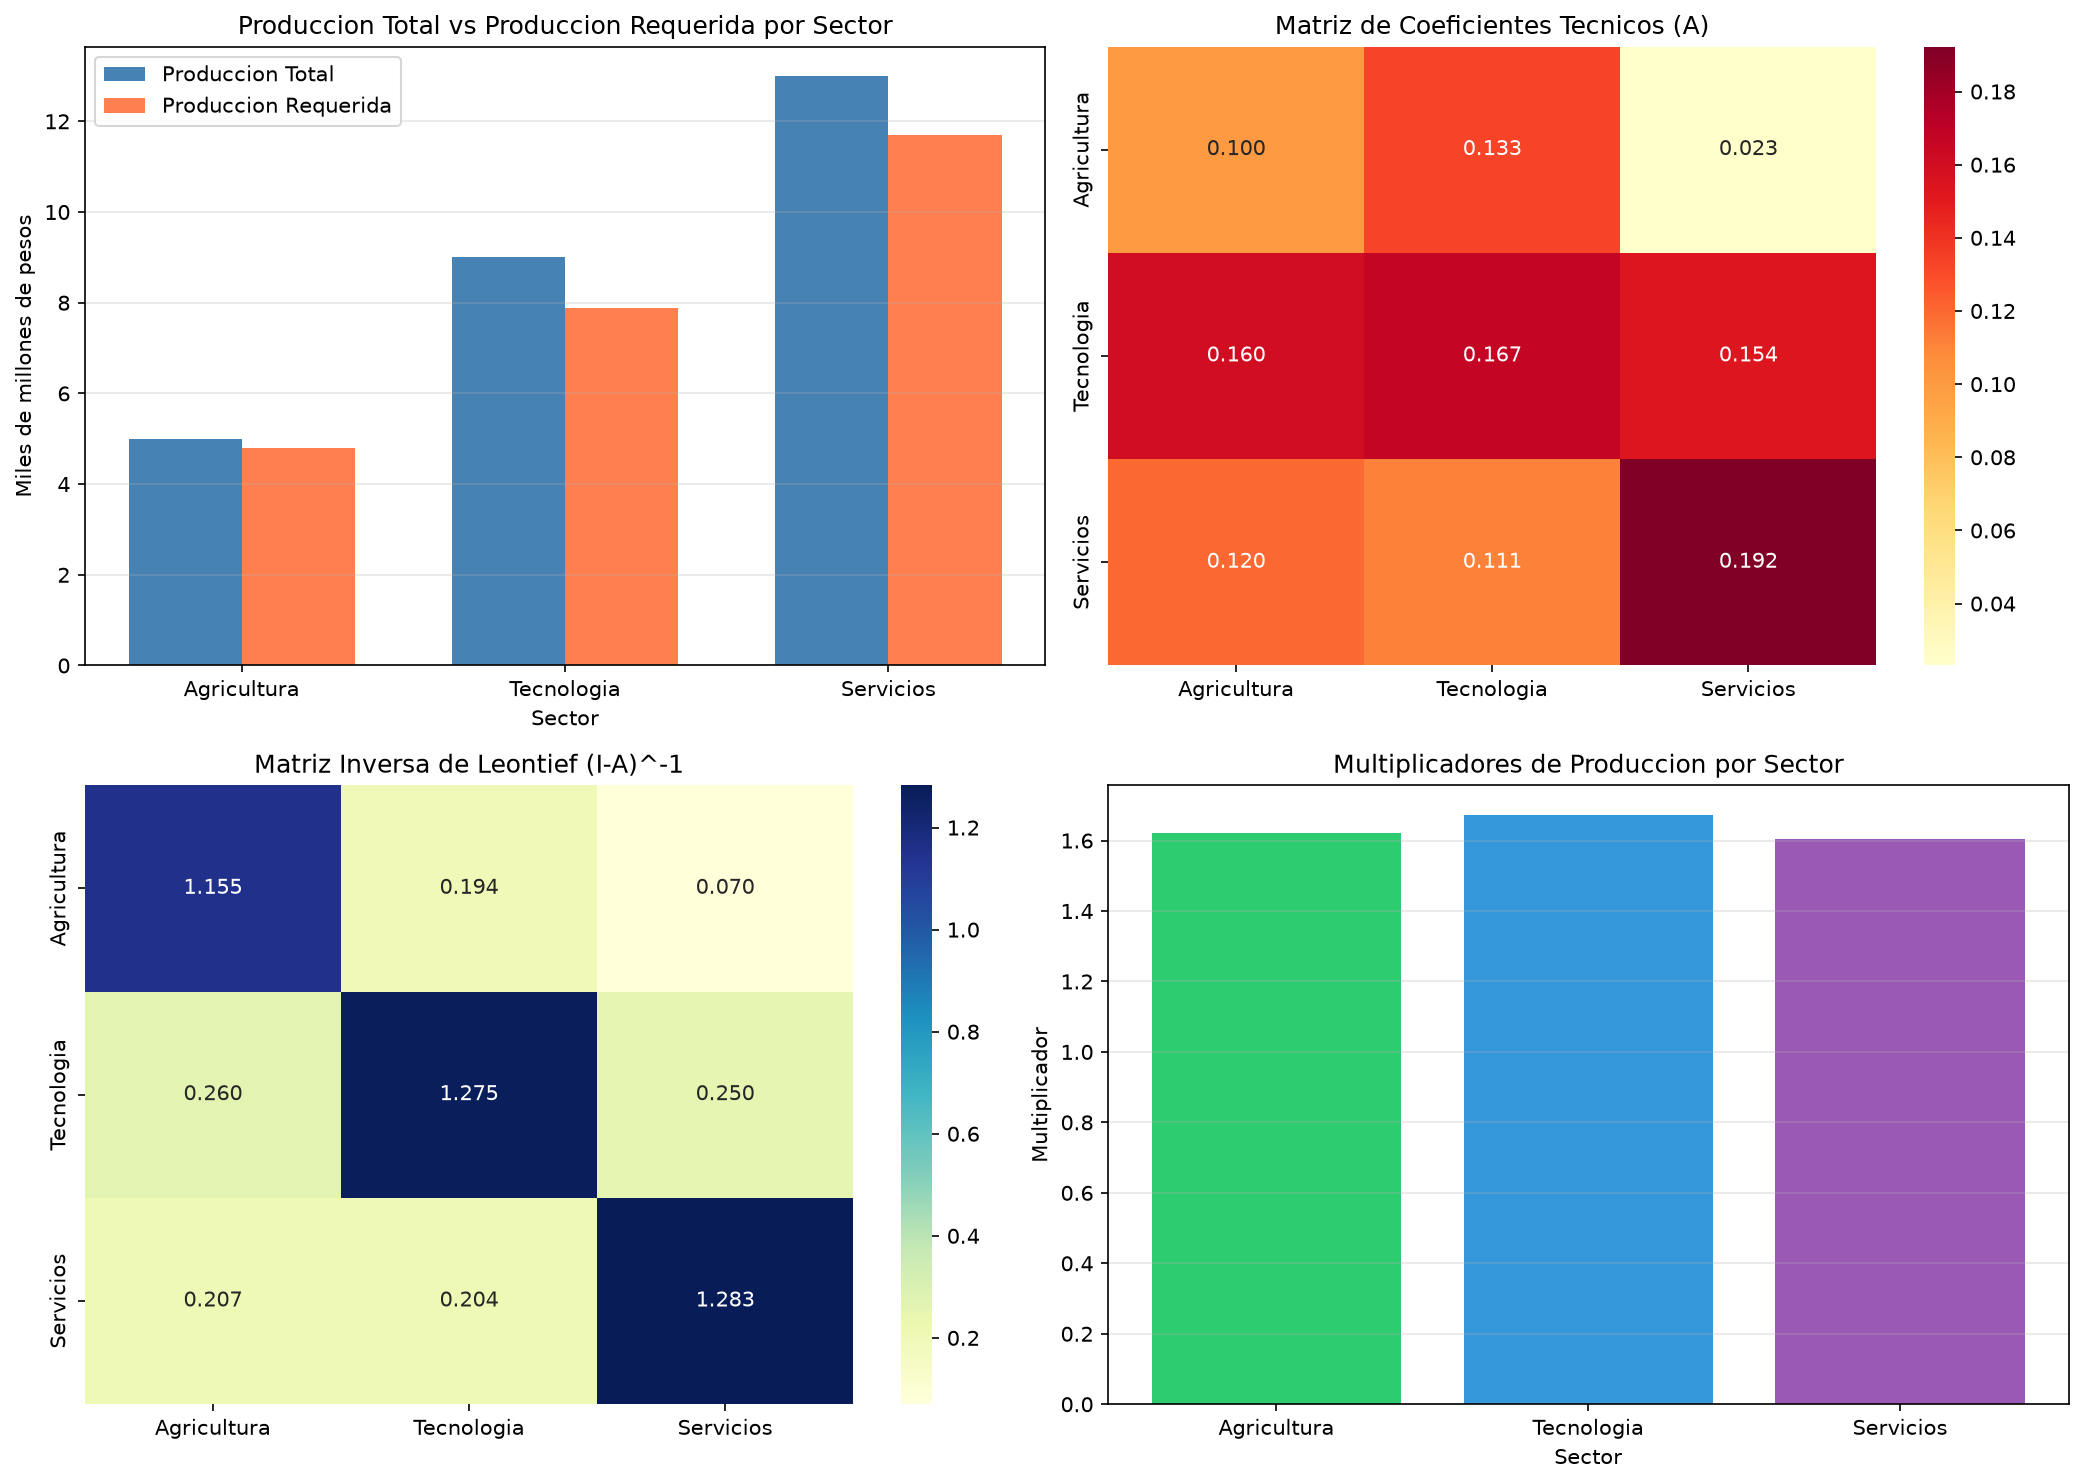
\includegraphics[width=0.9\textwidth]{ejercicio1_matriz_basica/resultados_leontieff.png}
\caption{Resultados de la Matriz de Leontief Básica}
\end{figure}

\clearpage
